%<dscrpt>Distance entre hauteurs d'un tétraèdre.</dscrpt>
\begin{figure}[h!t]
 \centering
 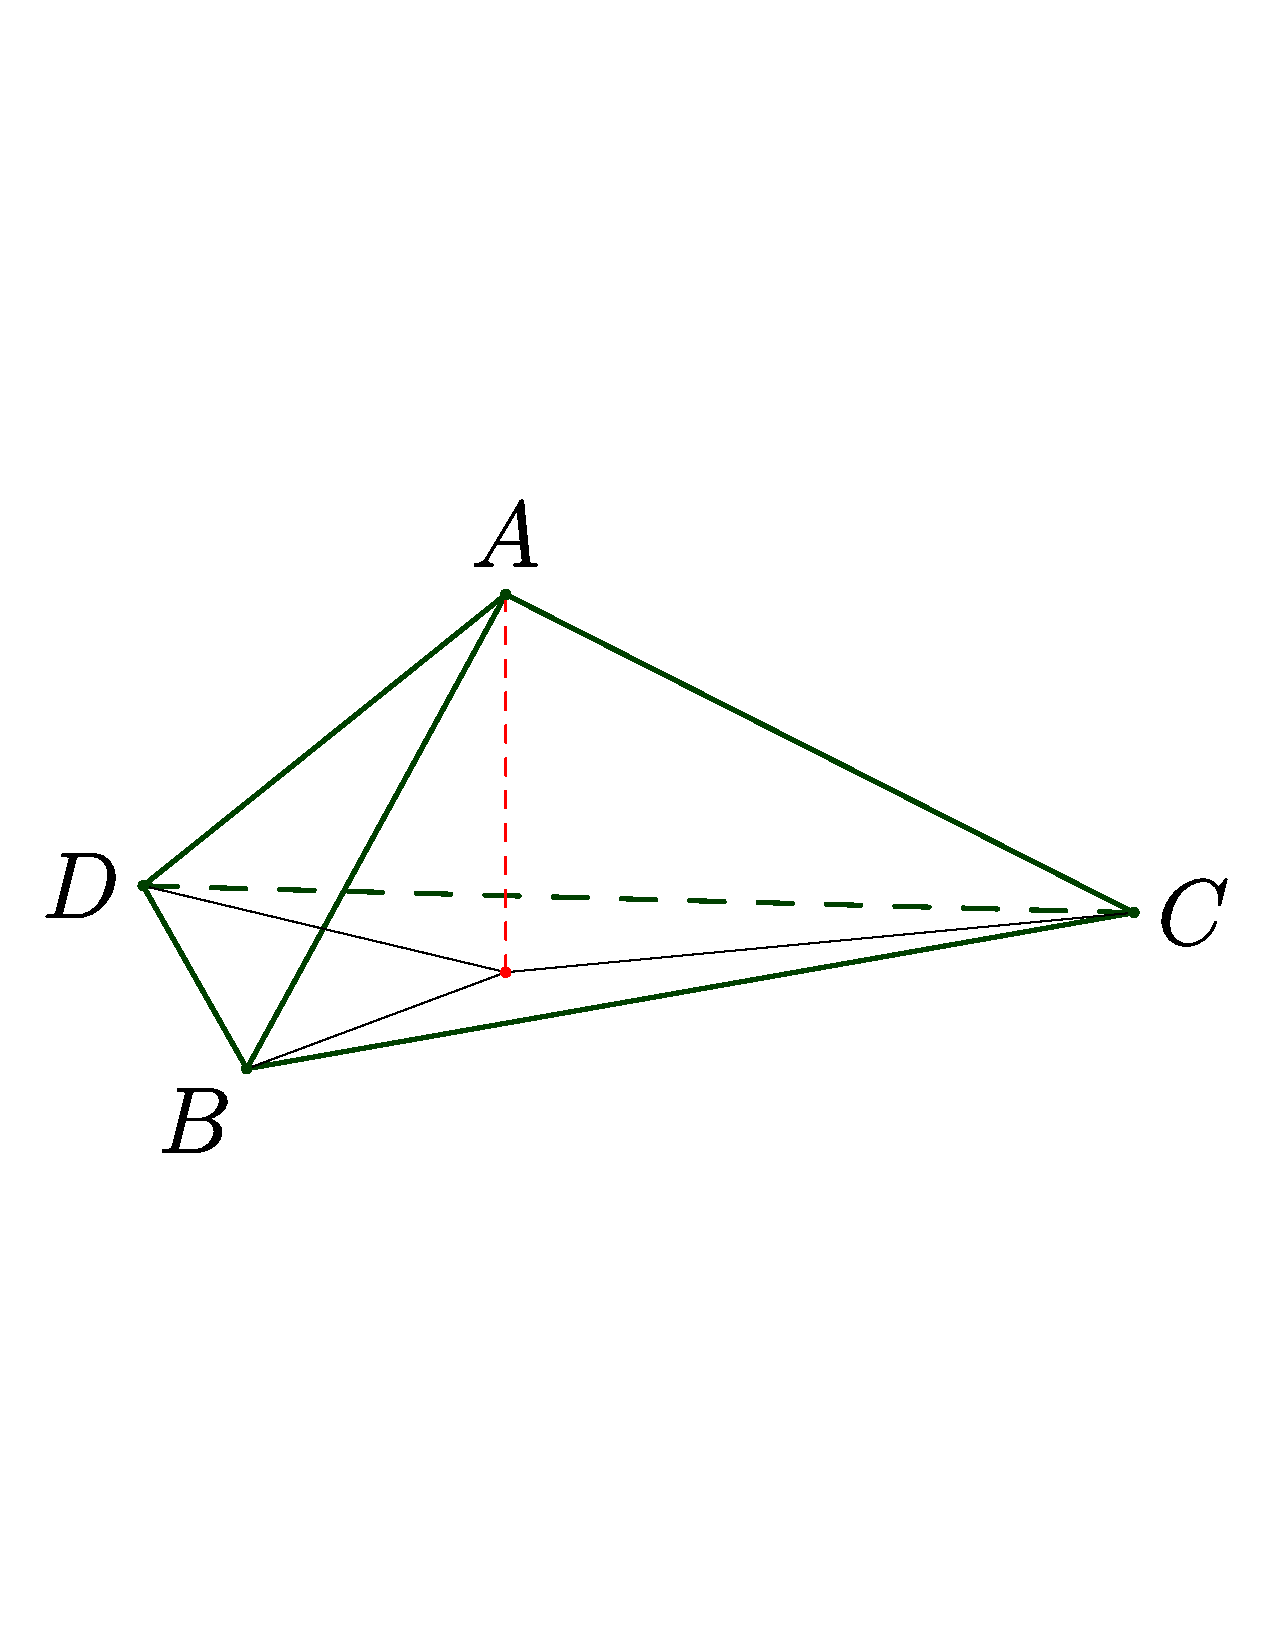
\includegraphics[width=7.5cm]{./Edishaut_1.pdf}
 % Edishaut_1.pdf: 0x0 pixel, 0dpi, 0.00x0.00 cm, bb=
 \caption{Hauteur d'un tétraèdre}
 \label{fig:Edishaut_1}
\end{figure}
Dans un espace euclidien orienté de dimension $3$, on considère $4$ points $A$, $B$, $C$, $D$ qui ne sont pas dans un même plan. On appelle \emph{hauteur} du tétraèdre qu'ils forment une droite passant par un des points $A$, $B$, $C$, $D$ et orthogonale au plan contenant les trois autres.
\begin{enumerate}
 \item Citer la formule du cours donnant la distance entre une droite $P +\Vect(\overrightarrow{u})$ et une droite $Q +\Vect(\overrightarrow{v})$.
 \item Simplifier
\begin{displaymath}
 \left(\overrightarrow{BC}\wedge \overrightarrow{BD} \right)
\wedge 
 \left(\overrightarrow{AC}\wedge \overrightarrow{AD} \right)
\end{displaymath}
sous la forme $\lambda \overrightarrow{u}$ où $\lambda$ et un réel et $\overrightarrow{u}$ un vecteur s'exprimant simplement en fonction de $A$, $B$, $C$, $D$.
\item Montrer que la distance entre les hauteurs issues de $A$ et de $B$ est de la forme $d\cos \delta$ où $d$ est la longueur d'une arête (à préciser) du tétraedre et $\delta$ un écart angulaire entre deux vecteurs (à préciser).
\item Donner une condition nécessaire et suffisante pour que les quatre hauteurs d'un tétraèdre se coupent deux à deux. Montrer que lorsque cette condition est réalisée, les hauteurs se coupent au même point.
\item On se donne trois points $B$, $C$, $D$ non algnés. Existe-t-il toujours un point $A$ tel que les quatre hauteur du tétraèdre $A$, $B$, $C$, $D$ se coupent ? Si oui où doit-il se trouver ? 
\end{enumerate}
